\section{Introduction}
\label{sec:introduction}
Intelligent information systems increasingly turn machine-produced information into persistent operational records through human review. Document intelligence and data curation illustrate a consequential case: a reviewer corrects a proposed value before authorizing its admission. Such a correction creates an authorization problem that the final record cannot reveal. A correct final value does not establish which machine proposal was preserved, which value the human authorized, or whether the admitted candidate was the exact instance reviewed.

Consider a record whose quantity is 90. A recognizer proposes 100, and a reviewer authorizes 101. Admission must retain the machine proposal 100 while committing the human-authorized value 101; an unchanged batch-code field must retain its earlier source. The proposal explains the origin of the correction, whereas the authorization permits the committed value. Overwriting the proposal collapses these roles and can falsely attribute the corrected value to the machine. Correction requires the relation to permit
\begin{equation}
x_c\neq x_a.
\label{eq:intro-correction}
\end{equation}

A further distinction survives even when values and review context agree. Two persisted extraction attempts can have the same proposal, record, field, evidence, expected version, and retained review context, yet remain different candidate instances. Reviewing one does not authorize the other under an instance-accountability policy. \emph{Equal-valued candidate substitution} exposes this difference without relying on a changed result or context mismatch. Candidate identity then becomes part of the integrity condition for authoritative admission: it identifies the object to which authorization applies.

We call this requirement \emph{candidate-bound authorization}. For corrected AI-derived updates, it binds the human's explicit authorized value to the exact persisted candidate while preserving the original proposal. The resulting admission relation connects
\begin{equation}
\begin{aligned}
\textit{exact candidate}
&\rightarrow\textit{candidate-bound authorization}\\
&\rightarrow\textit{explicit authorized value}\\
&\rightarrow\textit{fresh authoritative predecessor}\\
&\rightarrow\textit{complete successor and total field sources}.
\end{aligned}
\label{eq:admission-chain}
\end{equation}
Changed fields acquire transitions carrying their authorization; unchanged fields retain their exact prior sources. These bindings make the correction accountable both at commit and through subsequent queries.

\noindent\begin{minipage}{\textwidth}
We make three contributions:
\begin{description}[leftmargin=0pt,labelsep=0.5em,topsep=3pt,itemsep=0pt,parsep=0pt]
\item[C1:] \textbf{A correction-specific integrity requirement and admission relation.}
We formalize candidate-bound authorization and connect proposal preservation, explicit human value authority, predecessor freshness, complete successors, and total field sources in an executable contract.
\item[C2:] \textbf{A characterization of failure-distinguishing information.}
We identify five classes: candidate identity/context, proposal/authorized-value roles, freshness, successor completeness, and field-source attribution. Safe/unsafe paired histories show how omitting each class makes different authority outcomes observationally indistinguishable. Proposition~1 states the formal scope of this characterization.
\item[C3:] \textbf{Cross-representation realization and a decisive policy separator.}
An independently written exact-binding event journal and the relational reference agree on all 165 corresponding cases. Fifteen equal-valued substitutions separate both from context approval. Review-session controls locate the request-to-review and presentation boundaries; operational workloads characterize the cost of enforcing and querying the relation.
\end{description}
\end{minipage}

The gap concerns this end-to-end relation. Transactions can commit a substituted candidate atomically; freshness checks can validate its predecessor; provenance can record its effects; and approval can authorize matching content. None of those conditions, by itself, establishes that the admitted instance is the one reviewed. Existing mechanisms provide the means to enforce the relation, but its authorization target and correction semantics must be specified explicitly.


The central finding is an authorization distinction, not a preference for one storage design. Sections~2--6 position, specify, and check the relation; Sections~7--8 evaluate its policy separator, review boundary, and operational costs. Section~9 develops implications and trust boundaries. Figure~1 illustrates Correction and field lineage.

\begin{figure}[!htbp]
\centering
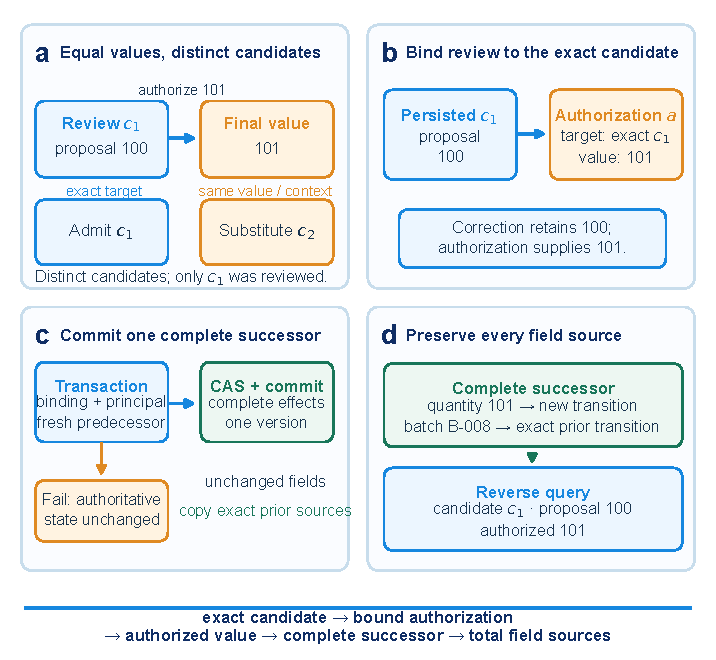
\includegraphics[width=0.975\textwidth]{Fig1.pdf}
\caption{The admission relation preserves both the reviewed instance and the original proposal through Correction. (a) Equal-valued candidates remain distinct authorization targets; (b) the authorized correction retains the proposal; (c) failed admission leaves authoritative state unchanged; (d) changed and unchanged fields retain their respective sources. Values illustrate a constructed example. Diagram preparation assisted by OpenAI Codex; image-generation prototype use is disclosed in Statements and Declarations}
\label{fig:admission-workflow}
\end{figure}
